{\usebackgroundtemplate{
    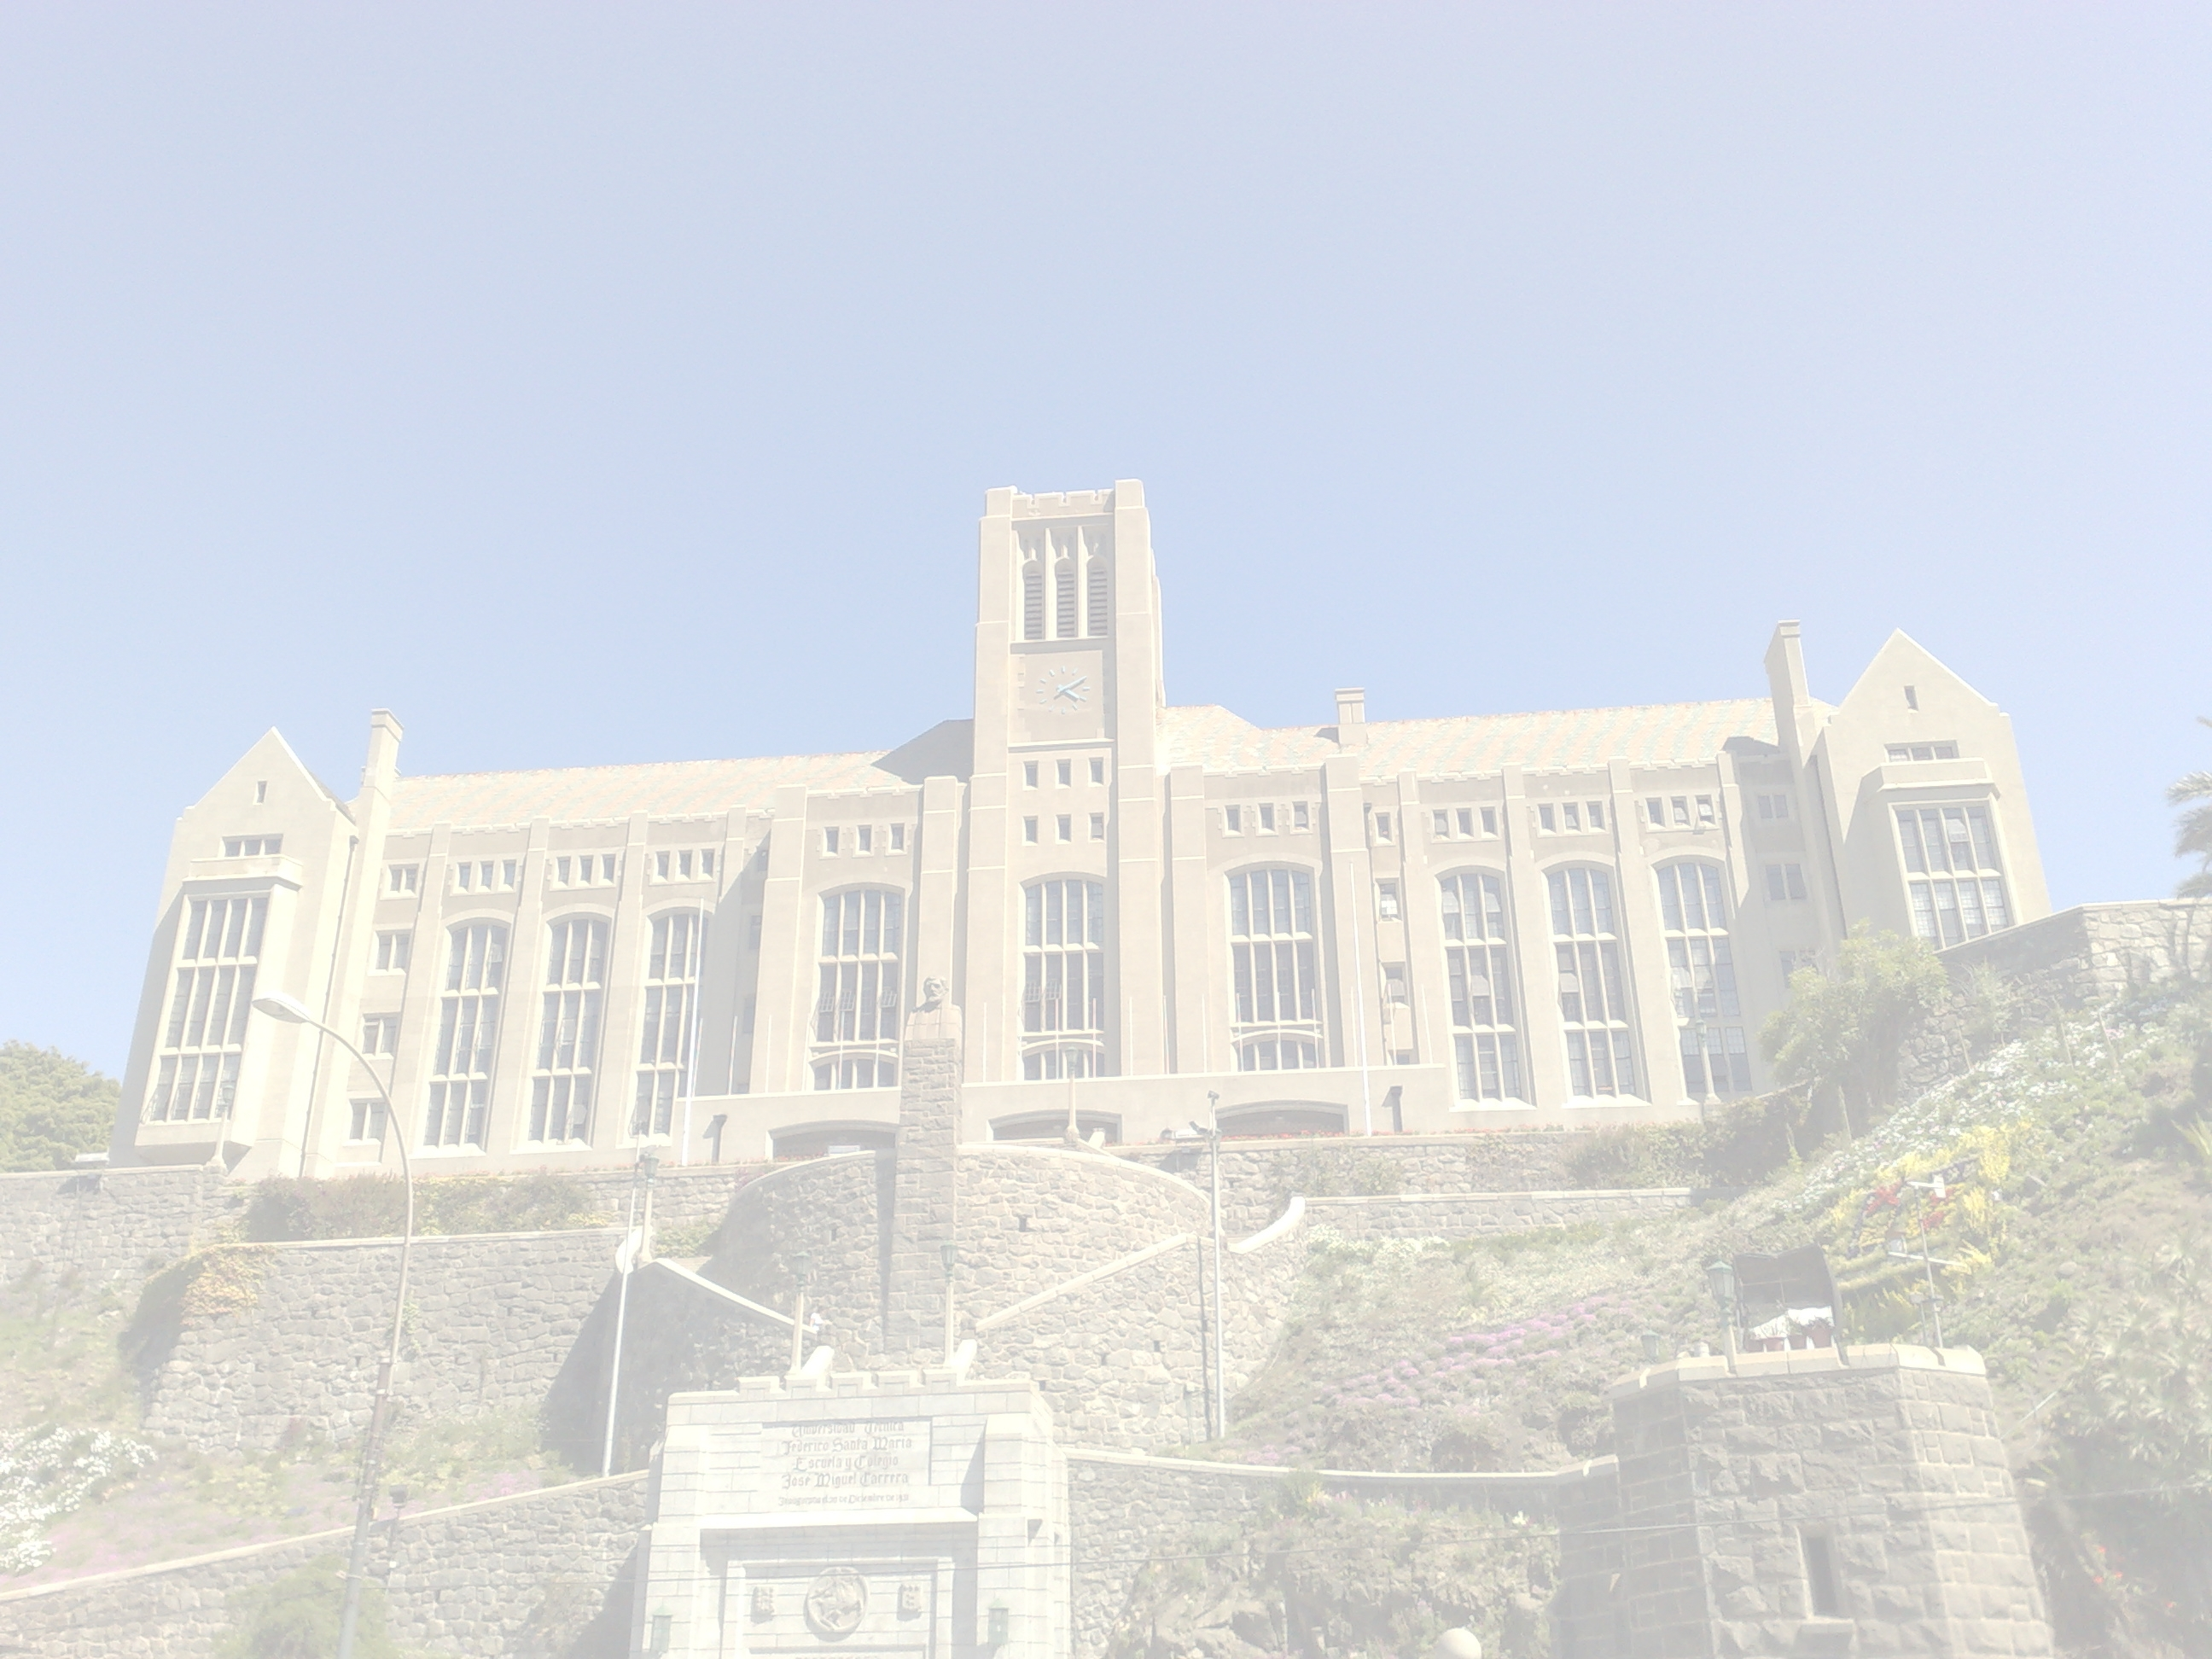
\includegraphics[width=\paperwidth,
      height=\paperheight]{Pict/UTFSM-30.jpg}
  }
  \begin{frame}
    \titlepage
  \end{frame}
}

\begin{frame}
  \frametitle{Geometrical Objects}

  \begin{description}
  \item [Scalars] Described through a {\it magnitud}
    \begin{align*}
      \phi \in \K\quad (\Z,\R,\C)
    \end{align*}
  \item [Vectors] Quantity endowed with {\it magnitude} and {\it direction}
    \begin{align*}
      \vec{V} = V^i \vb{i}\quad\to\quad V^i
    \end{align*}
    \begin{alertblock}{Einstein's sum convention}
      Repeated indices, positioned one upstairs and other downstairs, implies sum over all possible values of the index. Summed indices are dummy.
    \end{alertblock}
  \item [``Matrices''] ``Array'' (or vector) of vectors?
    \begin{align*}
      M =
      \begin{pmatrix}
        M_{11}& \cdots & M_{1n}\\
        \vdots & & \vdots\\
        M_{m1}&\cdots& M_{mn}
      \end{pmatrix}
      \quad&\to\quad M=M^{ij}\(\vb{i}\otimes\vb{j}\)\\
      &\to\quad M^{ij}
    \end{align*}
  \end{description}
\end{frame}

\begin{frame}
  \frametitle{Operations on Vectors}
  Let $\vec{V},\vec{W},\vec{U}$ be vectors and $\lambda$ a scalar.
  \begin{columns}[t]
    \column{.45\textwidth}
    {\small
      \begin{itemize}
      \item {\bf Addition}:
        \begin{align*}
          \vec{V}+\vec{W} = \(V^i +W^i\)\vb{i}
        \end{align*}
      \item {\bf Product with a scalar}
        \begin{align*}
          \lambda\vec{V}=\(\lambda V^i\)\vb{i}
        \end{align*}
      \item {\bf Scalar product of vectors}
        \begin{align*}
          \vec{V}\cdot\vec{W} = \delta_{ij}V^i W^j
        \end{align*}
      \item {\bf Vector product of vectors}
        \begin{align*}
          \vec{V}\times\vec{W} = \epsilon_{ijk}\fb{i}V^j W^k
        \end{align*}
      \end{itemize}
    }
    \column{.45\textwidth}
    \begin{alertblock}{Special Objects}
      {\bf Kr\"onecker delta}:
      \begin{align*}
        \delta_{ij} =
        \begin{cases}
          1 & i=j\\
          0 & \text{otherwise}
        \end{cases}
      \end{align*}

      {\bf Levi-Civita epsilon}:
      \begin{align*}
        \epsilon_{ijk} =
        \begin{cases}
          1 & \binom{123}{ijk}\text{ is even}\\
          -1 & \binom{123}{ijk}\text{ is odd}\\
          0 & \text{otherwise}
        \end{cases}
      \end{align*}
    \end{alertblock}
  \end{columns}
\end{frame}

\begin{frame}[t]
  \frametitle{Upper and Lower Indices}
  \begin{columns}
    \column{.45\textwidth}
    \begin{center}
      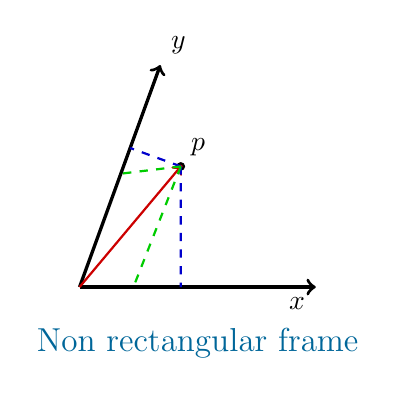
\begin{tikzpicture}
        % Definition
        \pgfmathsetmacro{\rp}{2}
        \pgfmathsetmacro{\th}{50}
        \pgfmathsetmacro{\ph}{20}
        \pgfmathsetmacro{\xa}{\rp*cos(\th)}
        \pgfmathsetmacro{\xb}{\rp*sin(90-\th-\ph)}
        \pgfmathsetmacro{\yb}{\rp*sin(\th)}
        \pgfmathsetmacro{\ya}{\rp*cos(90-\th-\ph)}

        % Coordinates
        \coordinate (O) at (0,0);
        \coordinate (P) at (\th:\rp cm);

        % Draw the frame
        \draw[very thick,->] (O) -- (0:3cm) node[anchor=north east] {$x$};
        \draw[very thick,->] (O) -- (90-\ph:3cm) node[anchor= south west] {$y$};

        % Draw point  with line
        \draw[fill=red!80!black,thick]  (P) circle (.4mm) node[anchor=south west] {$p$};
        \draw[color=red!80!black,thick,->] (O) -- (P);

        % Draw projections
        \draw[thick,dashed,color=blue!80!black] (P) -- (\xa,0);
        \draw[dashed,thick,color=blue!80!black] (P) -- (90-\ph:\ya);
         \draw[dashed,thick,color=green!80!black] (P) -- (\xb,0);
        \draw[dashed,thick,color=green!80!black] (P) -- (90-\ph:\yb);

        % Title
        \node[anchor=north,color=green!40!blue] at (current bounding box.south) {{\large Non rectangular frame}};       
      \end{tikzpicture}
    \end{center}    
    \column{.45\textwidth}
    \begin{itemize}
    \item There are two possible choices.
    \item One of them represented by {\it upper} index.
    \item the other represented by {\it lower} index.
    \end{itemize}

    \begin{block}{Vectors and Covectors}
      A customary notation is to said that, \alert{vectors} do have upper indices, while \alert{covectors} have lower indices.
    \end{block}
  \end{columns}
\end{frame}

\begin{frame}
  \frametitle{Operations on Matrices}
  Let $\vec{M},\vec{T}$ be matrices and $\lambda$ a scalar.
  \begin{columns}[t]
    \column{.45\textwidth}
    {\small
      \begin{itemize}
      \item {\bf Addition}:
        \begin{align*}
          {M}+{T} = \(M^{ij} +T^{ij}\)\vb{i}\otimes\vb{j}
        \end{align*}
      \item {\bf Product with a scalar}
        \begin{align*}
          \lambda{M}=\(\lambda M^{ij}\)\vb{i}\otimes\vb{j}
        \end{align*}
      %% \item {\bf Scalar product of vectors}
      %%   \begin{align*}
      %%     \vec{V}\cdot\vec{W} = \delta_{ij}V^i W^j
      %%   \end{align*}
      \item {\bf Matrix product}
        \begin{align*}
          MT = M^{ij}\delta_{jk} T^{kl} \equiv M^i{}_j T^{j l}
        \end{align*}
      \end{itemize}
    }
    \column{.45\textwidth}
    \begin{alertblock}{Lowering and Raising indices}
      The  Kr\"onecker delta, or a metric in general, is used for raising or lowering indices, defined as
      \begin{align*}
        V_i &\equiv \delta_{ij}V^j\\
        V^i &\equiv \delta^{ij}V_j
      \end{align*}
    \end{alertblock}
  \end{columns}
\end{frame}


\begin{frame}[t]
  \frametitle{Transformations}
    \begin{center}
      \begin{tikzpicture}
        % Definitions
        \pgfmathsetmacro{\rp}{2}
        \pgfmathsetmacro{\be}{50}
        \pgfmathsetmacro{\th}{20}
        \pgfmathsetmacro{\px}{\rp*cos(\be)}
        \pgfmathsetmacro{\py}{\rp*sin(\be)}
        \pgfmathsetmacro{\al}{\be-\th}
        \pgfmathsetmacro{\xa}{\rp*cos(\be)}
        \pgfmathsetmacro{\ya}{\rp*sin(\be)}
        \pgfmathsetmacro{\xb}{\rp*cos(\al)}
        \pgfmathsetmacro{\yb}{\rp*sin(\al)}

        % Coordinates
        \coordinate (O) at (0,0);
        \coordinate (P) at (\px,\py);

        % Draw O coordinate system
        \draw[thick,->] (O) -- (0:3cm) node[anchor=north west] {$x$};
        \draw[thick,->] (O) -- (90:3cm) node[anchor=south] {$y$};

        % Draw O' coordinate system
        \draw[thick,->,color=blue] (O) -- (\th:3cm) node[anchor=north west] {$x$};
        \draw[thick,->,color=blue] (O) -- (\th+90:3cm) node[anchor=south] {$y$};

        % Draw the point with line
        \draw[fill=red!80!black,thick]  (P) circle (.4mm) node[anchor=south west] {$p$};
        \draw[color=red!80!black,thick,->] (O) -- (P);

        % Projection to O system
        \draw[thin,dashed] (P) -- (\xa,0) node[anchor=north] {$x_p$};
        \draw[thin,dashed] (P) -- (0,\ya) node[anchor=east] {$y_p$};

        % Projection to O' system
        \draw[thin,dashed,color=blue] (P) -- (\th:\xb) node[anchor=north west] {${x'}_p$};
        \draw[thin,dashed,color=blue] (P) -- (\th+90:\yb) node[anchor=north east] {${y'}_p$};

        % Arcs
        \draw[left color=red!30, right color=red!15,draw=red!60!black] (O) -- (\th:8mm) arc (\th:\be:8mm)  -- cycle;
        \draw (O) +(35:8mm) node[color=red,anchor=south west]  {$\alpha$};
        \draw[left color=blue!30, right color=blue!15,draw=blue!60!black] (O) -- (0:8mm) arc (0:\th:8mm)  -- cycle;
        \node[anchor=west,color=blue] at (\th*2/3:8mm) {$\theta$};

        % Information box
        \draw[xshift=35mm,yshift=15mm] node[right,text width=6cm,rounded corners,fill=red!10,draw=red!40!yellow,inner sep=1ex] {
          \begin{align*}
            x_p = & r_p \cos(\theta+\alpha) \\
            = &x'_p \cos(\theta) - y'_p\sin(\theta)\\
            y_p = & r_p \sin(\theta+\alpha) \\
            = & x'_p \sin(\theta) - y'_p\cos(\theta)
          \end{align*}
        };
      \end{tikzpicture}
    \end{center}
  \begin{columns}
    \column{.5\textwidth}
    {\small
      \begin{align*}
        \begin{pmatrix}
          x'_p\\ y'_p
        \end{pmatrix} = 
        \begin{pmatrix}
          \cos(\theta) & \sin(\theta)\\
          -\sin(\theta) & \cos(\theta)
        \end{pmatrix}
        \begin{pmatrix}
          x_p\\ y_p
        \end{pmatrix}
      \end{align*}
    }
    \column{.5\textwidth}
    In general,
    \begin{align*}
      X' = R(\theta) X,
    \end{align*}
    where $\{R(\theta)\}$ form a \alert{group} of transformations
  \end{columns}
\end{frame}

\begin{frame}[t]
  \frametitle{Definitions from transformations}
  It make sense to define \alert{geometrical objects} depending of their transformation rules of a given group.
  \begin{definition}%{Scalar}
    A {\bf \alert{scalar}} (of a group) is the quantity that remain invariable under the transformation group.
    \begin{align*}
      \Phi' = \Phi
    \end{align*}
  \end{definition}
  \pause
  \begin{alertblock}{R\^ole of group theory}
    \begin{itemize}%[<+->]
    \item One might assign a geometrical object to any irrep of a group.
    \item A scalar is the corresponding to the trivial representation.
    \item A vector is the corresponding to the \alert{fundamental} representation.
    \end{itemize}
  \end{alertblock}
\end{frame}


\begin{frame}
  \frametitle{Definition of Vector}
  \begin{definition}
    A \alert{vector} (of a group) is the quantity that transform under the fundamental representation of the group, i.e.,
    \begin{align*}
      V' = \Lambda V.
    \end{align*}
  \end{definition}
  \begin{alertblock}{Warning}
    \begin{itemize}
    \item $\R^n$ is so simple that is not a good example.
    \item $\R^n$ is the basis for more complex examples.
    \item There are more than `a' vector space.
    \end{itemize}
  \end{alertblock}
\end{frame}


\begin{frame}
  \frametitle{Graphical Representation of Scalar Transf.}
  \begin{center}
    \begin{tikzpicture}
      % Definitions
        \pgfmathsetmacro{\rp}{2}
        \pgfmathsetmacro{\be}{50}
        \pgfmathsetmacro{\th}{20}
        \pgfmathsetmacro{\px}{\rp*cos(\be)}
        \pgfmathsetmacro{\py}{\rp*sin(\be)}
        \pgfmathsetmacro{\al}{\be-\th}
        \pgfmathsetmacro{\xa}{\rp*cos(\be)}
        \pgfmathsetmacro{\ya}{\rp*sin(\be)}
        \pgfmathsetmacro{\xb}{\rp*cos(\al)}
        \pgfmathsetmacro{\yb}{\rp*sin(\al)}

        % Coordinates
        \coordinate (O) at (0,0);
        \coordinate (P) at (\px,\py);

        % Draw O coordinate system
        \draw[thick,->] (O) -- (0:3cm) node[anchor=north west] {$x$};
        \draw[thick,->] (O) -- (90:3cm) node[anchor=south] {$y$};

        % Draw O' coordinate system
        \draw[thick,->,color=blue] (O) -- (\th:3cm) node[anchor=north west] {$x$};
        \draw[thick,->,color=blue] (O) -- (\th+90:3cm) node[anchor=south] {$y$};

        % Draw the point with line
        \draw[fill=red!80!black,thick]  (P) circle (.4mm) node[anchor=south west] {$p$};
        \draw[color=red!80!black,thick,->] (O) -- (P);

        % Projection to O system
        \draw[thin,dashed] (P) -- (\xa,0) node[anchor=north] {$x_p$};
        \draw[thin,dashed] (P) -- (0,\ya) node[anchor=east] {$y_p$};

        % Projection to O' system
        \draw[thin,dashed,color=blue] (P) -- (\th:\xb) node[anchor=north west] {${x'}_p$};
        \draw[thin,dashed,color=blue] (P) -- (\th+90:\yb) node[anchor=north east] {${y'}_p$};

        % Information box
        \draw[xshift=35mm,yshift=15mm] node[right,text width=6cm,rounded corners,fill=red!10,draw=red!40!yellow,inner sep=1ex] {
          In $S$ there is a function $f(x)$, while in $S'$ there is a $f'(x')$.
          \begin{align*}
            f'(x') = f'\(\Lambda x\) = & f(x)\\
            \text{or}\quad f'\(x\) = & f\(\Lambda^{-1} x\).
          \end{align*}
        };
    \end{tikzpicture}
  \end{center}
\end{frame}

\begin{frame}
  \frametitle{Graphical Representation of Vector Transf.}
  \begin{center}
    \begin{tikzpicture}
      % Definitions
        \pgfmathsetmacro{\rp}{2}
        \pgfmathsetmacro{\be}{50}
        \pgfmathsetmacro{\th}{20}
        \pgfmathsetmacro{\px}{\rp*cos(\be)}
        \pgfmathsetmacro{\py}{\rp*sin(\be)}
        \pgfmathsetmacro{\al}{\be-\th}
        \pgfmathsetmacro{\xa}{\rp*cos(\be)}
        \pgfmathsetmacro{\ya}{\rp*sin(\be)}
        \pgfmathsetmacro{\xb}{\rp*cos(\al)}
        \pgfmathsetmacro{\yb}{\rp*sin(\al)}

        % Coordinates
        \coordinate (O) at (0,0);
        \coordinate (P) at (\px,\py);

        % Draw O coordinate system
        \draw[thick,->] (O) -- (0:3cm) node[anchor=north west] {$x$};
        \draw[thick,->] (O) -- (90:3cm) node[anchor=south] {$y$};

        % Draw O' coordinate system
        \draw[thick,->,color=blue] (O) -- (\th:3cm) node[anchor=north west] {$x$};
        \draw[thick,->,color=blue] (O) -- (\th+90:3cm) node[anchor=south] {$y$};

        % Draw the point with line
        \draw[fill=red!80!black,thick]  (P) circle (.4mm) node[anchor=south west] {$p$};
        \draw[color=red!80!black,thick,->] (O) -- (P);

        % Projection to O system
        \draw[thin,dashed] (P) -- (\xa,0) node[anchor=north] {$x_p$};
        \draw[thin,dashed] (P) -- (0,\ya) node[anchor=east] {$y_p$};

        % Projection to O' system
        \draw[thin,dashed,color=blue] (P) -- (\th:\xb) node[anchor=north west] {${x'}_p$};
        \draw[thin,dashed,color=blue] (P) -- (\th+90:\yb) node[anchor=north east] {${y'}_p$};

        % Draw the vector
        \draw[very thick,color=yellow!75!black,->] (P) -- +(110:1cm) node[anchor=south west,color=black] {$\vec{V}$};

        % Information box
        \draw[xshift=35mm,yshift=15mm] node[right,text width=6cm,rounded corners,fill=red!10,draw=red!40!yellow,inner sep=1ex] {
          In $S$ there is a vector $\vec{V}(x)$, while in $S'$ there is a $\vec{V}'(x')$.
          \begin{align*}
            \vec{V}'(x') = \vec{V}'\(\Lambda x\) = & \Lambda\vec{V}(x)\\
            \text{or}\quad \vec{V}'\(x\) = & \Lambda\vec{V}\(\Lambda^{-1} x\).
          \end{align*}
        };
    \end{tikzpicture}
  \end{center}
\end{frame}

\begin{frame}
  \frametitle{Resum\`e of transformations}
  All geometrical objects are defined though their transformations. Therefore, given a group of transformations, one define: (below $p$ is a geometrical point of the space.)
  \begin{itemize}
  \item {\bf Scalars} 
    \begin{align*}
      \phi'(p) = \phi(p)
    \end{align*}
    \item {\bf Vectors} 
    \begin{align*}
      V'(p) &= \Lambda\,V(p)\\
      \(V'\)^i &= \Lambda^i{}_j V^j
    \end{align*}
    \item {\bf Matrices} 
    \begin{align*}
      M'(p) &= \Lambda\Lambda\,M(p)\\
      \(M'\)^{ij} &= \Lambda^i{}_k\Lambda^j{}_l M^{kl}
    \end{align*}
  \end{itemize}
\end{frame}



\begin{frame}
  \frametitle{Tensors}
  \begin{definition}
    A \alert{\bf Tensor} is a multilinear geometrical  object which transform as,
    \begin{align*}
      {T'}^{a_1\cdots a_p}{}_{b_1\cdots b_q} =  \Lambda^{a_1}_{m_1} \cdots  \Lambda^{a_p}_{m_p}(\Lambda^{-1})^{n_1}_{b_1} \cdots (\Lambda^{-1})^{n_q}_{b_q} {T}^{m_1\cdots m_p}{}_{n_1\cdots n_q},
    \end{align*}
    i.e., a `vector' transformation per index.
  \end{definition}
  \begin{itemize}
  \item Tensors are classified by their indices, $\binom{p}{q}$-tensors.
  \item Scalars are $\binom{0}{0}$-tensors.
  \item Vectors are $\binom{1}{0}$-tensors, while covectors are $\binom{0}{1}$-tensors.
  \item Metrics are $\binom{0}{2}$-tensors.
  \end{itemize}
\end{frame}

{\usebackgroundtemplate{
    
\includegraphics[width=\paperwidth,
      height=\paperheight]{Pict/Q2.pdf}
  }
\begin{frame}
  \frametitle{\alert{WORKED EXAMPLES}}
  Given a coordinate transformation.
  \begin{itemize}[<+-|alert@+>]
  \item  Show how do the vector basis, $\{\vb{i}\}$, transform.
  \item Show how do the partial derivatives transform. 
  \end{itemize}

  \onslide<3>{
  Therefore, partial derivatives respect to the coordinates are a suitable choice of vector basis.
  }
\end{frame}
}

\begin{frame}
  \frametitle{BE AWARE OF ...}
  \begin{alertblock}{WARNING}
    Not every object with indices is a  tensor
  \end{alertblock}
  \begin{example}
    The derivative of a vector is not a tensor,
    \begin{align*}
      \partial_a V^b \;\to \;{\partial'}_a {V'}^b = (\Lambda^{-1})_a^c\, \Lambda^b_d\partial_c\, V^d + \alert{(\Lambda^{-1})_a^c\,\partial_c(\Lambda^b_d) \,V^d }.
    \end{align*}

    In general, it is true for any kind of tensors.
  \end{example}
\end{frame}


\begin{frame}
  \frametitle{Distance and Metric}
  \begin{columns}
    \column{.45\textwidth}
    Given two points $p_1$ and $p_2$, the (Euclidean) distance between the points is
    \begin{align*}
      ds^2 &= \(x_2-x_1\)^2 +\(y_2-y_1\)^2  \\
      &= \delta_{ij} \(\Delta x^i\)\(\Delta x^j\)
    \end{align*}
    \column{.45\textwidth}
    %--------- Draw of the distance between two dots
    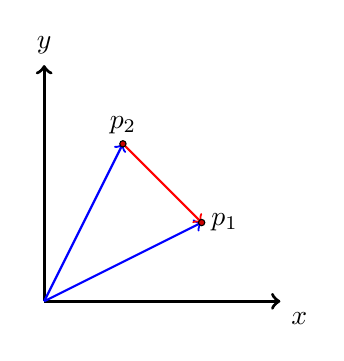
\begin{tikzpicture}
    % Coordinates
    \coordinate (O) at (0,0);
    \coordinate (xa) at (3,0);
    \coordinate (ya) at (0,3);
    \coordinate (p1) at (2,1);
    \coordinate (p2) at (1,2);

    % Draw the coordinate system
    \draw[very thick,->] (O) -- (xa) node[anchor=north west] {$x$};
    \draw[very thick,->] (O) -- (ya) node[anchor=south] {$y$};

    % Draw vectors
    \draw[color=blue,->,thick] (O) -- (p1);
    \draw[color=blue,->,thick] (O) -- (p2);
    \draw[color=red,->,thick] (p2) -- (p1);

    % Draw the points
    \draw[fill=red!80!black] (p1) circle (.4mm) node[anchor=west] {$p_1$};
    \draw[fill=red!80!black] (p2) circle (.4mm) node[anchor=south] {$p_2$};
    \end{tikzpicture}
  \end{columns}

  \begin{alertblock}{Kr\"onercker delta as a metric}
    The geometrical object which is used to define the distance between two points is called \alert{metric}, and the Kr\"onercker delta plays the r\^ole of Euclidean metric.

In general, the metric is denoted by the letter $g$.
  \end{alertblock}
\end{frame}

\begin{frame}
  \frametitle{More about the metric}
  \begin{columns}[t]
    \column{.45\textwidth}
    The metric
    \begin{itemize}
    \item  is defined to be a $\binom{0}{2}$-tensor.
    \item relate the vectors and covectors.
    \item define distance.
    \item with upper indices denotes the inverse of the metric.
    \item with mixed indices is \alert{always} a Kr\"onecker delta.
    \end{itemize}
    \column{.45\textwidth}
    \begin{block}{Metric and vector basis}
      Given a set of vector basis, $\{\vb{i}\}$, the metric can be obtain though the relation,
      \begin{align*}
        g_{i j} = \vb{i}\cdot \vb{j}
      \end{align*}
    \end{block}
  \end{columns}
\end{frame}

{\usebackgroundtemplate{
    
\includegraphics[width=\paperwidth,
      height=\paperheight]{Pict/Q2.pdf}
  }
\begin{frame}
  \frametitle{\alert{WORKED EXAMPLES}}
  Given a coordinate transformation, 
  \begin{itemize}
  \item How do the metric transform?
  \item Find the metric in polar coordinates.
  \end{itemize}
\end{frame}
}

\begin{frame}
  \frametitle{Decomposition of Tensors}
  \textbf{Symmetrisation}
  \begin{align*}
    T_{(a_1\cdots a_n)} = \frac{1}{n!}\sum_{\text{perm.}}T_{\sigma(a_1)\cdots \sigma(a_n)}
  \end{align*}

  \textbf{Anti-symmetrisation}
  \begin{align*}
    T_{(a_1\cdots a_n)} = \frac{1}{n!}\sum_{\text{perm.}}\(-1\)^{\abs{\sigma}}T_{\sigma(a_1)\cdots \sigma(a_n)}
  \end{align*}
\end{frame}

{\usebackgroundtemplate{
    
\includegraphics[width=\paperwidth,
      height=\paperheight]{Pict/Q2.pdf}
  }
\begin{frame}
  \frametitle{\alert{WORKED EXAMPLES}}
  
  \begin{itemize}
  \item Given a general $\binom{0}{2}$-tensor, show that it is the sum of its symmetric and anti-symmetric parts.
  \item Is the above also true for $\binom{0}{3}$-tensor.
  \end{itemize}
 
\end{frame}
}
